% === LaTeX Figure Includes ===
% Auto-generated by paper-figure skill

% === Fig 2: Beta Ablation ===
\begin{figure}[t]
    \centering
    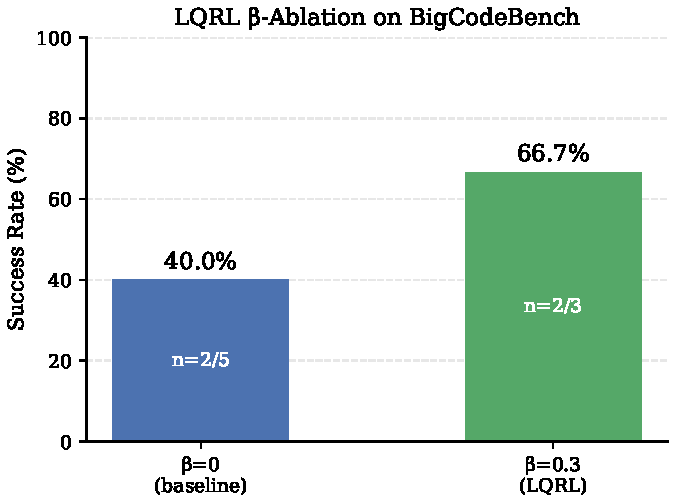
\includegraphics[width=0.48\textwidth]{figures/fig2_ablation.pdf}
    \caption{BigCodeBench success rate comparison between baseline Q-learning (β=0) and LQRL (β=0.3). Small sample sizes (n=5 and n=3) due to compute constraints; larger evaluation needed for statistically significant conclusions.}
    \label{fig:ablation}
\end{figure}

% === TABLE 1: Main Results ===
% See figures/TABLE_main_results.tex for standalone table

% === MANUAL FIGURES (need manual creation) ===
% Fig 1 (Hero): System overview — architecture diagram showing standard Q-learning vs LQRL
%   - Left panel: Task Fail → Content Improve → Q decreases
%   - Right panel: Task Fail → Content Improve → r_learning evaluated → Q maintained
%   - Use draw.io, Figma, or TikZ to create
%
% Fig 3: Q-value entropy over task number (planned)
%
% Fig 4: Multi-benchmark comparison (planned)
